\documentclass[]{book}
\usepackage{lmodern}
\usepackage{amssymb,amsmath}
\usepackage{ifxetex,ifluatex}
\usepackage{fixltx2e} % provides \textsubscript
\ifnum 0\ifxetex 1\fi\ifluatex 1\fi=0 % if pdftex
  \usepackage[T1]{fontenc}
  \usepackage[utf8]{inputenc}
\else % if luatex or xelatex
  \ifxetex
    \usepackage{mathspec}
  \else
    \usepackage{fontspec}
  \fi
  \defaultfontfeatures{Ligatures=TeX,Scale=MatchLowercase}
\fi
% use upquote if available, for straight quotes in verbatim environments
\IfFileExists{upquote.sty}{\usepackage{upquote}}{}
% use microtype if available
\IfFileExists{microtype.sty}{%
\usepackage{microtype}
\UseMicrotypeSet[protrusion]{basicmath} % disable protrusion for tt fonts
}{}
\usepackage[margin=1in]{geometry}
\usepackage{hyperref}
\hypersetup{unicode=true,
            pdftitle={Tidy time series forecasting with fable},
            pdfborder={0 0 0},
            breaklinks=true}
\urlstyle{same}  % don't use monospace font for urls
\usepackage{natbib}
\bibliographystyle{plainnat}
\usepackage{color}
\usepackage{fancyvrb}
\newcommand{\VerbBar}{|}
\newcommand{\VERB}{\Verb[commandchars=\\\{\}]}
\DefineVerbatimEnvironment{Highlighting}{Verbatim}{commandchars=\\\{\}}
% Add ',fontsize=\small' for more characters per line
\usepackage{framed}
\definecolor{shadecolor}{RGB}{248,248,248}
\newenvironment{Shaded}{\begin{snugshade}}{\end{snugshade}}
\newcommand{\AlertTok}[1]{\textcolor[rgb]{0.94,0.16,0.16}{#1}}
\newcommand{\AnnotationTok}[1]{\textcolor[rgb]{0.56,0.35,0.01}{\textbf{\textit{#1}}}}
\newcommand{\AttributeTok}[1]{\textcolor[rgb]{0.77,0.63,0.00}{#1}}
\newcommand{\BaseNTok}[1]{\textcolor[rgb]{0.00,0.00,0.81}{#1}}
\newcommand{\BuiltInTok}[1]{#1}
\newcommand{\CharTok}[1]{\textcolor[rgb]{0.31,0.60,0.02}{#1}}
\newcommand{\CommentTok}[1]{\textcolor[rgb]{0.56,0.35,0.01}{\textit{#1}}}
\newcommand{\CommentVarTok}[1]{\textcolor[rgb]{0.56,0.35,0.01}{\textbf{\textit{#1}}}}
\newcommand{\ConstantTok}[1]{\textcolor[rgb]{0.00,0.00,0.00}{#1}}
\newcommand{\ControlFlowTok}[1]{\textcolor[rgb]{0.13,0.29,0.53}{\textbf{#1}}}
\newcommand{\DataTypeTok}[1]{\textcolor[rgb]{0.13,0.29,0.53}{#1}}
\newcommand{\DecValTok}[1]{\textcolor[rgb]{0.00,0.00,0.81}{#1}}
\newcommand{\DocumentationTok}[1]{\textcolor[rgb]{0.56,0.35,0.01}{\textbf{\textit{#1}}}}
\newcommand{\ErrorTok}[1]{\textcolor[rgb]{0.64,0.00,0.00}{\textbf{#1}}}
\newcommand{\ExtensionTok}[1]{#1}
\newcommand{\FloatTok}[1]{\textcolor[rgb]{0.00,0.00,0.81}{#1}}
\newcommand{\FunctionTok}[1]{\textcolor[rgb]{0.00,0.00,0.00}{#1}}
\newcommand{\ImportTok}[1]{#1}
\newcommand{\InformationTok}[1]{\textcolor[rgb]{0.56,0.35,0.01}{\textbf{\textit{#1}}}}
\newcommand{\KeywordTok}[1]{\textcolor[rgb]{0.13,0.29,0.53}{\textbf{#1}}}
\newcommand{\NormalTok}[1]{#1}
\newcommand{\OperatorTok}[1]{\textcolor[rgb]{0.81,0.36,0.00}{\textbf{#1}}}
\newcommand{\OtherTok}[1]{\textcolor[rgb]{0.56,0.35,0.01}{#1}}
\newcommand{\PreprocessorTok}[1]{\textcolor[rgb]{0.56,0.35,0.01}{\textit{#1}}}
\newcommand{\RegionMarkerTok}[1]{#1}
\newcommand{\SpecialCharTok}[1]{\textcolor[rgb]{0.00,0.00,0.00}{#1}}
\newcommand{\SpecialStringTok}[1]{\textcolor[rgb]{0.31,0.60,0.02}{#1}}
\newcommand{\StringTok}[1]{\textcolor[rgb]{0.31,0.60,0.02}{#1}}
\newcommand{\VariableTok}[1]{\textcolor[rgb]{0.00,0.00,0.00}{#1}}
\newcommand{\VerbatimStringTok}[1]{\textcolor[rgb]{0.31,0.60,0.02}{#1}}
\newcommand{\WarningTok}[1]{\textcolor[rgb]{0.56,0.35,0.01}{\textbf{\textit{#1}}}}
\usepackage{longtable,booktabs}
\usepackage{graphicx,grffile}
\makeatletter
\def\maxwidth{\ifdim\Gin@nat@width>\linewidth\linewidth\else\Gin@nat@width\fi}
\def\maxheight{\ifdim\Gin@nat@height>\textheight\textheight\else\Gin@nat@height\fi}
\makeatother
% Scale images if necessary, so that they will not overflow the page
% margins by default, and it is still possible to overwrite the defaults
% using explicit options in \includegraphics[width, height, ...]{}
\setkeys{Gin}{width=\maxwidth,height=\maxheight,keepaspectratio}
\usepackage[normalem]{ulem}
% avoid problems with \sout in headers with hyperref:
\pdfstringdefDisableCommands{\renewcommand{\sout}{}}
\IfFileExists{parskip.sty}{%
\usepackage{parskip}
}{% else
\setlength{\parindent}{0pt}
\setlength{\parskip}{6pt plus 2pt minus 1pt}
}
\setlength{\emergencystretch}{3em}  % prevent overfull lines
\providecommand{\tightlist}{%
  \setlength{\itemsep}{0pt}\setlength{\parskip}{0pt}}
\setcounter{secnumdepth}{5}
% Redefines (sub)paragraphs to behave more like sections
\ifx\paragraph\undefined\else
\let\oldparagraph\paragraph
\renewcommand{\paragraph}[1]{\oldparagraph{#1}\mbox{}}
\fi
\ifx\subparagraph\undefined\else
\let\oldsubparagraph\subparagraph
\renewcommand{\subparagraph}[1]{\oldsubparagraph{#1}\mbox{}}
\fi

%%% Use protect on footnotes to avoid problems with footnotes in titles
\let\rmarkdownfootnote\footnote%
\def\footnote{\protect\rmarkdownfootnote}

%%% Change title format to be more compact
\usepackage{titling}

% Create subtitle command for use in maketitle
\newcommand{\subtitle}[1]{
  \posttitle{
    \begin{center}\large#1\end{center}
    }
}

\setlength{\droptitle}{-2em}

  \title{Tidy time series forecasting with fable}
    \pretitle{\vspace{\droptitle}\centering\huge}
  \posttitle{\par}
    \author{}
    \preauthor{}\postauthor{}
      \predate{\centering\large\emph}
  \postdate{\par}
    \date{2019-05-23}

\usepackage{booktabs}
\usepackage{amsthm}
\makeatletter
\def\thm@space@setup{%
  \thm@preskip=8pt plus 2pt minus 4pt
  \thm@postskip=\thm@preskip
}
\makeatother

\begin{document}
\maketitle

{
\setcounter{tocdepth}{1}
\tableofcontents
}
\hypertarget{forecasting-with-fable}{%
\chapter{Forecasting with fable}\label{forecasting-with-fable}}

The \texttt{fable} package is a tidy renovation of the \href{https://github.com/robjhyndman/forecast/}{forecast} package, and it explores new interfaces for modelling and subsequent analysis in R. For users experienced with the tidyverse, modelling in R can be a jarring experience. Models in R can be difficult to work with as there is little standardisation in model object structures and interfaces. This is partially alleviated from tidy modelling packages such as \href{https://github.com/tidymodels/broom/}{broom} (and \href{https://github.com/business-science/sweep}{sweep} for time series) which can be used to extract key features from model objects in suitable formats for tidy workflows.

The existing integration of modelling and the tidyverse is especially problematic for time series, as the input data structure (ts) is inherently untidy. Much like \href{https://pkg.earo.me/tsibble/}{tsibble} implements tidy time series data, the \texttt{fable} package applies tidyverse principles to time series modelling, making the forecasting workflow seamlessly integrate with other \texttt{tidyverse} packages.

The design choices around \texttt{fable} prioritise the user interface, allowing complicated models to be estimated using common statistical terminology. It intentionally abstracts away from the complications of programming to allow users to focus on the model(s) that they are estimating rather than how they are coding it.

\hypertarget{background}{%
\section{Background}\label{background}}

The ideas presented in this resource are subject to revision, as the development of these tools are still experimental. This text aims to consolidate the information currently dispersed in the \texttt{fable} package documentation, wiki pages, issues, and emails in a way that is more accessible to the wider community. Hopefully this firstly helps us better design and plan the workflow of tidy forecasting, and invite external opinions to ensure that \texttt{fable} works well with the existing tidy modelling developments.

\hypertarget{tsibble}{%
\chapter{Tidy time series}\label{tsibble}}

\hypertarget{ts}{%
\section{ts}\label{ts}}

Time series data structures in R vary substantially, however most time series models make use of the \texttt{ts} object structure from the \texttt{stats} package. This object concisely stores the time series index using three `time series parameters' (\texttt{tsp}): \texttt{start}, \texttt{frequency}, and \texttt{end}. For most time series tools (such as \texttt{arima}, \texttt{ets}, \texttt{stl}) this structural information is sufficient, however it lacks details that are present in modern time series datasets:

\begin{itemize}
\tightlist
\item
  Multiple seasonality
\item
  Irregular observations
\item
  Exogenous information
\item
  Many time series (that differ in length)
\end{itemize}

In many senses this structure is limited, and inconsistent with the \href{https://cran.r-project.org/web/packages/tidyr/vignettes/tidy-data.html}{tidy data principles}:

\begin{itemize}
\tightlist
\item
  Non-rectangular index structure
\item
  Wide-format for keyed data (\texttt{mts})
\item
  Unnatural index format for importing data
\item
  Difficulty working with tidyverse tools
\end{itemize}

\hypertarget{tsibble-1}{%
\section{tsibble}\label{tsibble-1}}

The \href{https://github.com/tidyverts/tsibble}{tsibble package} by \href{https://github.com/earowang}{Earo Wang} provides a tidy data structure for time series, and is well described in her \href{https://pkg.earo.me/tsibble/articles/intro-tsibble.html}{introductory vignette}.

This data structure is sufficiently flexible to support the future of time series modelling tools (such as \texttt{tbats}, \texttt{fasster} and \texttt{prophet}). Beyond the data tidying and transformation tools that the package provides, the object also includes valuable structural information (\texttt{index} and \texttt{key}) for time series modelling.

\hypertarget{index}{%
\subsection{index}\label{index}}

The index is essential for modelling as it can be used to identify the frequency and regularity of the observations. By storing a standard \texttt{datetime} object within the dataset, it makes irregular time series modelling possible. It also allows a more flexible specification of seasonal frequency (see \protect\hyperlink{interface}{seasonal period}) that is easier to specify for the end user (a very \href{https://robjhyndman.com/hyndsight/seasonal-periods/}{common difficulty} when constructing \texttt{ts} objects).

\hypertarget{key}{%
\subsection{key}\label{key}}

Keys are used within tsibble to uniquely identify related time series in a tidy structure. They are also useful for identifying relational structures between each time series. This is especially useful for \href{https://otexts.org/fpp2/hierarchical.html}{forecast reconciliation}, where a hierarchical or grouped structure is imposed on a set of forecasts to impose relational constraints (typically aggregation). Keys within tsibble can be either nested (hierarchical) or crossed (grouped), and can be directly used to reconcile forecasts. This structure also has purpose for univariate models, as it allows \protect\hyperlink{advanced}{batch forecasting} to be applied across many time series.

\hypertarget{model}{%
\chapter{Model basics}\label{model}}

The \href{https://github.com/tidyverts/fablelite}{fablelite} package provides a set of tools for creating models that work well together. These tools aim to simplify model development and encourage a consistent interface across many model types. By developing a model with fablelite, complexity introduced by batch forecasting and \protect\hyperlink{advanced}{advanced functionality} is handled automatically. This should allow model developers to focus on implementing model specific functionality.

The model function is expected to accept a tsibble and model formula, and return a fitted model stored as a mable.

\hypertarget{interface}{%
\section{Model specification}\label{interface}}

A consistent interface across models is essential.

\hypertarget{model-formula}{%
\section{Model formula}\label{model-formula}}

fable introduces the formula based model specification that is familiar in cross-sectional models to time series. This allows an interface for concise and human readable model specifications. Additionally, this change allows a more flexible specification of transformations, and model elements. A typical model formula may look like this:

\begin{Shaded}
\begin{Highlighting}[]
\KeywordTok{log}\NormalTok{(y) }\OperatorTok{~}\StringTok{ }\KeywordTok{trend}\NormalTok{() }\OperatorTok{+}\StringTok{ }\KeywordTok{season}\NormalTok{(}\DataTypeTok{period =} \StringTok{"day"}\NormalTok{) }\OperatorTok{+}\StringTok{ }\NormalTok{x}
\end{Highlighting}
\end{Shaded}

Like \texttt{lm()} and other cross-sectional model interfaces, the left hand side of the formula defines the response. fable extends this standard usage by supporting transformations of any type. In the above example, a \texttt{log} transformation has been used on the response variable, \texttt{y}. Unlike other models, the transformation specified in formula's LHS will be automatically inverted, and used for automatic back-transformation of your forecasts and fitted values. For more details on how transformations work within fable, you can refer to the transformations vignette: \texttt{vignette("transformations",\ package="fable")}

On the right hand side of the formula, we define the specials used for the model. Specifying the RHS is optional, and any required specials that are omitted will be included using their defaults (allowing for automatic model selection). In the above formula, we have included a trend, a daily seasonal pattern and exogenous regressor \texttt{x}. The specials that are supported will vary between each model function, and the available specials are (should be) documented under the ``Model Formula'' section of the help file.

\hypertarget{selection-parameters}{%
\section{Selection parameters}\label{selection-parameters}}

\hypertarget{optimisation-parameters}{%
\section{Optimisation parameters}\label{optimisation-parameters}}

\hypertarget{computational-parameters}{%
\section{Computational parameters}\label{computational-parameters}}

\hypertarget{accessing-model-elements}{%
\chapter{Accessing model elements}\label{accessing-model-elements}}

\hypertarget{display}{%
\section{Display}\label{display}}

The \texttt{print} and \texttt{summary} methods are standard displays for fitted models. The \texttt{print} method typically displays a limited amount of key information, such as the model that was fit, and the estimated coefficients. The \texttt{summary} function extends the \texttt{print} method with a more detailed summary of fit, which may include measures for goodness of fit, and significance of model terms.

As fable naturally supports batch/multiple forecasting, the print method is standardised for any number of models. A very short model specific display can be defined using the \texttt{model\_sum} generic, which is shown in the mable.

\begin{Shaded}
\begin{Highlighting}[]
\KeywordTok{library}\NormalTok{(tsibbledata)}
\NormalTok{UKLungDeaths <-}\StringTok{ }\KeywordTok{as_tsibble}\NormalTok{(}\KeywordTok{cbind}\NormalTok{(mdeaths, fdeaths), }\DataTypeTok{gather =} \OtherTok{FALSE}\NormalTok{)}
\end{Highlighting}
\end{Shaded}

\begin{verbatim}
## Warning: Argument `gather` is deprecated, please use `pivot_longer`
## instead.
\end{verbatim}

\begin{Shaded}
\begin{Highlighting}[]
\NormalTok{ets_fit <-}\StringTok{ }\NormalTok{UKLungDeaths }\OperatorTok\StringTok{ }
\StringTok{  }\KeywordTok{model}\NormalTok{(}\KeywordTok{ETS}\NormalTok{(mdeaths))}
\end{Highlighting}
\end{Shaded}

\begin{verbatim}
## # A mable: 1 x 1
##   `ETS(mdeaths)`
##   <model>       
## 1 <ETS(M,A,A)>
\end{verbatim}

The summary method can then be used to reveal more information about this model, such as fitted parameters and goodness of fit. Ideally this information would also be standardised into a tabular form for batch modelling, although this is currently not the case.

\begin{Shaded}
\begin{Highlighting}[]
\NormalTok{ets_fit }\OperatorTok\StringTok{ }
\StringTok{  }\NormalTok{summary}
\end{Highlighting}
\end{Shaded}

\begin{verbatim}
##        Length Class  Mode
## par     2     tbl_df list
## est     4     tbl_ts list
## fit     8     tbl_df list
## states 15     tbl_ts list
## spec    5     tbl_df list
\end{verbatim}

\hypertarget{fitted-values-and-residuals}{%
\section{Fitted values and residuals}\label{fitted-values-and-residuals}}

Accessors for fitted values and residuals return a tsibble containing the index from the original data, with a measured variables for \texttt{.fitted} values and \texttt{.resids}. If the mable contains more than one model, the resulting object maintains and respects the key structure.

\begin{Shaded}
\begin{Highlighting}[]
\NormalTok{ets_fit }\OperatorTok\StringTok{ }
\StringTok{  }\NormalTok{fitted}
\end{Highlighting}
\end{Shaded}

\begin{verbatim}
## # A tsibble: 72 x 3 [1M]
## # Key:       .model [1]
##    .model          index .fitted
##    <chr>           <mth>   <dbl>
##  1 ETS(mdeaths) 1974 Jan   2278.
##  2 ETS(mdeaths) 1974 Feb   2283.
##  3 ETS(mdeaths) 1974 Mar   2142.
##  4 ETS(mdeaths) 1974 Apr   1776.
##  5 ETS(mdeaths) 1974 May   1442.
##  6 ETS(mdeaths) 1974 Jun   1341.
##  7 ETS(mdeaths) 1974 Jul   1270.
##  8 ETS(mdeaths) 1974 Aug   1160.
##  9 ETS(mdeaths) 1974 Sep   1147.
## 10 ETS(mdeaths) 1974 Oct   1381.
## # ... with 62 more rows
\end{verbatim}

\begin{Shaded}
\begin{Highlighting}[]
\NormalTok{ets_fit }\OperatorTok\StringTok{ }
\StringTok{  }\NormalTok{residuals}
\end{Highlighting}
\end{Shaded}

\begin{verbatim}
## # A tsibble: 72 x 3 [1M]
## # Key:       .model [1]
##    .model          index   .resid
##    <chr>           <mth>    <dbl>
##  1 ETS(mdeaths) 1974 Jan -0.0633 
##  2 ETS(mdeaths) 1974 Feb -0.184  
##  3 ETS(mdeaths) 1974 Mar -0.124  
##  4 ETS(mdeaths) 1974 Apr  0.0569 
##  5 ETS(mdeaths) 1974 May  0.0346 
##  6 ETS(mdeaths) 1974 Jun -0.0689 
##  7 ETS(mdeaths) 1974 Jul  0.00764
##  8 ETS(mdeaths) 1974 Aug -0.0248 
##  9 ETS(mdeaths) 1974 Sep  0.0544 
## 10 ETS(mdeaths) 1974 Oct  0.0805 
## # ... with 62 more rows
\end{verbatim}

\hypertarget{broom-functionality}{%
\section{Broom functionality}\label{broom-functionality}}

Common features from a model can also be accessed using verbs from the \href{https://github.com/tidymodels/broom}{broom package}. Again, key structures that exist within the mable are respected.

\begin{Shaded}
\begin{Highlighting}[]
\NormalTok{ets_fit }\OperatorTok\StringTok{ }
\StringTok{  }\NormalTok{augment}
\end{Highlighting}
\end{Shaded}

\begin{verbatim}
## # A tsibble: 72 x 5 [1M]
## # Key:       .model [1]
##    .model          index mdeaths .fitted   .resid
##    <chr>           <mth>   <dbl>   <dbl>    <dbl>
##  1 ETS(mdeaths) 1974 Jan    2134   2278. -0.0633 
##  2 ETS(mdeaths) 1974 Feb    1863   2283. -0.184  
##  3 ETS(mdeaths) 1974 Mar    1877   2142. -0.124  
##  4 ETS(mdeaths) 1974 Apr    1877   1776.  0.0569 
##  5 ETS(mdeaths) 1974 May    1492   1442.  0.0346 
##  6 ETS(mdeaths) 1974 Jun    1249   1341. -0.0689 
##  7 ETS(mdeaths) 1974 Jul    1280   1270.  0.00764
##  8 ETS(mdeaths) 1974 Aug    1131   1160. -0.0248 
##  9 ETS(mdeaths) 1974 Sep    1209   1147.  0.0544 
## 10 ETS(mdeaths) 1974 Oct    1492   1381.  0.0805 
## # ... with 62 more rows
\end{verbatim}

\begin{Shaded}
\begin{Highlighting}[]
\NormalTok{ets_fit }\OperatorTok\StringTok{ }
\StringTok{  }\NormalTok{tidy}
\end{Highlighting}
\end{Shaded}

\begin{Shaded}
\begin{Highlighting}[]
\NormalTok{ets_fit }\OperatorTok\StringTok{ }
\StringTok{  }\NormalTok{glance}
\end{Highlighting}
\end{Shaded}

\begin{verbatim}
## # A tibble: 1 x 9
##   .model        sigma2 logLik   AIC  AICc   BIC    MSE   AMSE    MAE
##   <chr>          <dbl>  <dbl> <dbl> <dbl> <dbl>  <dbl>  <dbl>  <dbl>
## 1 ETS(mdeaths) 0.00905  -500. 1033. 1045. 1072. 24137. 23441. 0.0657
\end{verbatim}

\hypertarget{components}{%
\section{Components}\label{components}}

In many cases, a model can be used to extract features or components from data in a similar way to decomposition methods. We use the \texttt{components} verb to extract a tsibble of data features that have been extracted via modelling or decomposition.

State space models such as \texttt{ETS} are well suited to this functionality as the states often represent features of interest.

\begin{Shaded}
\begin{Highlighting}[]
\NormalTok{UKLungDeaths }\OperatorTok\StringTok{ }
\StringTok{  }\KeywordTok{model}\NormalTok{(}\KeywordTok{ETS}\NormalTok{(mdeaths)) }\OperatorTok\StringTok{ }
\StringTok{  }\NormalTok{components}
\end{Highlighting}
\end{Shaded}

\begin{verbatim}
## # A dable:                  84 x 7 [1M]
## # Key:                      .model [1]
## # ETS(M,A,A) Decomposition: mdeaths = (lag(level, 1) + lag(slope, 1) +
## #   lag(season, 12)) * (1 + remainder)
##    .model          index mdeaths level slope season remainder
##    <chr>           <mth>   <dbl> <dbl> <dbl>  <dbl>     <dbl>
##  1 ETS(mdeaths) 1973 Jan      NA    NA    NA   611.        NA
##  2 ETS(mdeaths) 1973 Feb      NA    NA    NA   620.        NA
##  3 ETS(mdeaths) 1973 Mar      NA    NA    NA   483.        NA
##  4 ETS(mdeaths) 1973 Apr      NA    NA    NA   122.        NA
##  5 ETS(mdeaths) 1973 May      NA    NA    NA  -207.        NA
##  6 ETS(mdeaths) 1973 Jun      NA    NA    NA  -304.        NA
##  7 ETS(mdeaths) 1973 Jul      NA    NA    NA  -370.        NA
##  8 ETS(mdeaths) 1973 Aug      NA    NA    NA  -476.        NA
##  9 ETS(mdeaths) 1973 Sep      NA    NA    NA  -485.        NA
## 10 ETS(mdeaths) 1973 Oct      NA    NA    NA  -246.        NA
## # ... with 74 more rows
\end{verbatim}

\begin{verbatim}
## Warning: Removed 11 rows containing missing values (geom_path).
\end{verbatim}

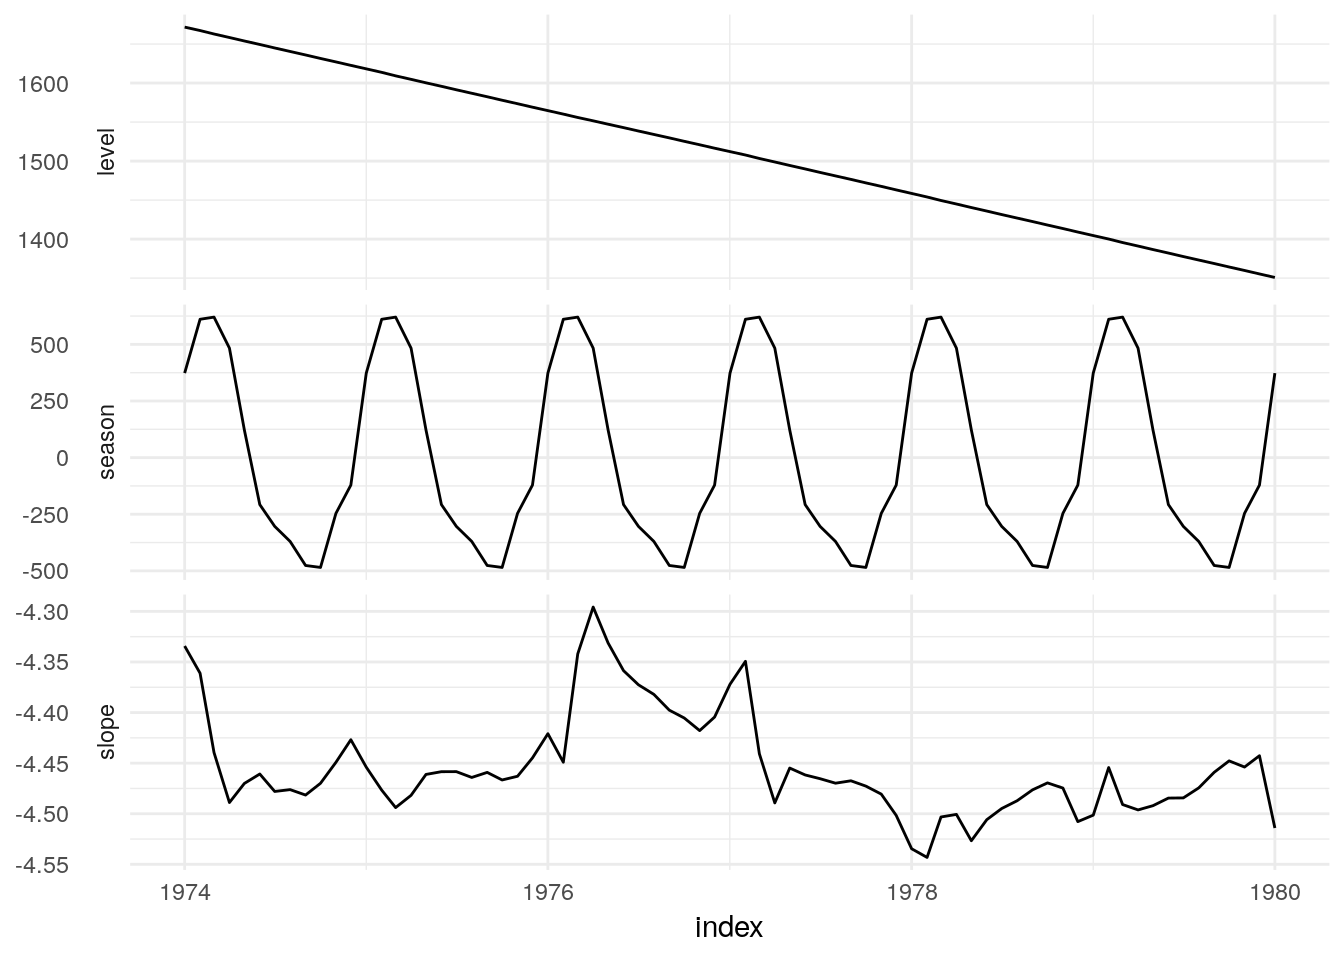
\includegraphics{tidy-forecasting_files/figure-latex/components-display-1.pdf}

It may also be worth storing how these components can be used to produce the response, which can be used for \href{https://mitchelloharawild.github.io/tidy-forecasting-principles/advanced.html\#decomposition}{decomposition modelling}.

\hypertarget{methods}{%
\chapter{Model methods}\label{methods}}

\hypertarget{interpolation}{%
\section{Interpolation}\label{interpolation}}

Models that can be estimated in the presence of missing values can often be used to interpolate the unknown values. Often interpolated values can be taken from model's fitted values, and some models may support more sophisticated interpolation methods.

The \href{https://github.com/robjhyndman/forecast/}{forecast package} provides the \texttt{na.interp} function for interpolating time series data, which uses linear interpolation for non-seasonal data, and STL decomposition for seasonal data.

Tidy time series tools should allow users to interpolate missing values using any appropriate model.

For example, the \texttt{tsibbledata::olympic\_running} dataset contains Olympic men's 400m track final winning times. The winning times for the 1916, 1940 and 1944 Olympics are missing from the dataset due to the World Wars.

\begin{verbatim}
## Warning: Removed 31 rows containing missing values (geom_point).
\end{verbatim}

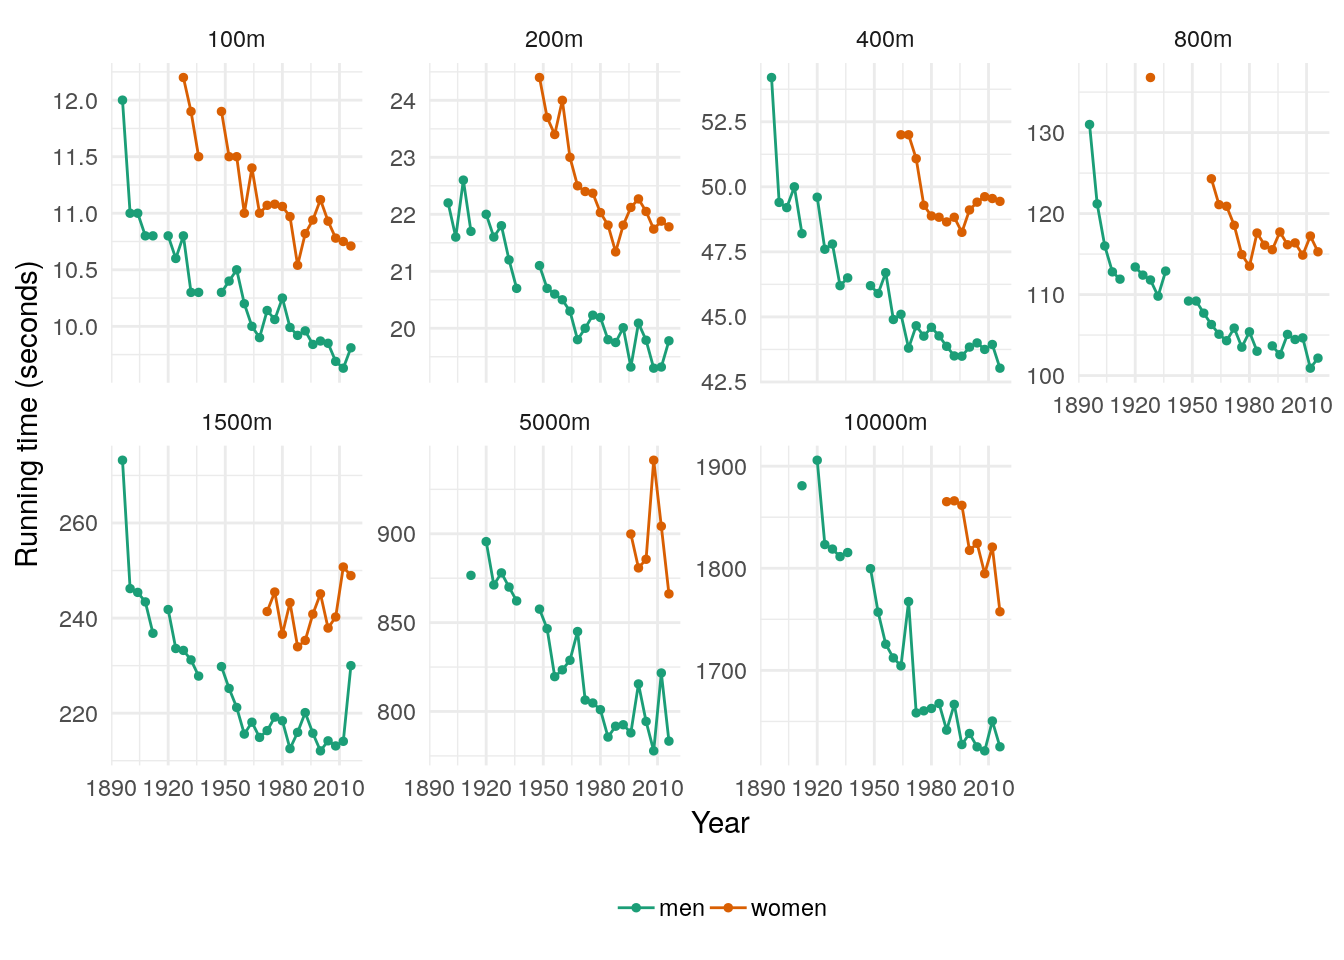
\includegraphics{tidy-forecasting_files/figure-latex/mens400-1.pdf}

We could then interpolate these missing values using the fitted values from a linear model with a trend:

\begin{Shaded}
\begin{Highlighting}[]
\NormalTok{olympic_running }\OperatorTok\StringTok{ }
\StringTok{  }\KeywordTok{model}\NormalTok{(}\DataTypeTok{lm =} \KeywordTok{TSLM}\NormalTok{(Time }\OperatorTok{~}\StringTok{ }\KeywordTok{trend}\NormalTok{())) }\OperatorTok\StringTok{ }
\StringTok{  }\KeywordTok{interpolate}\NormalTok{(olympic_running)}
\end{Highlighting}
\end{Shaded}

\begin{verbatim}
## # A tsibble: 312 x 4 [4Y]
## # Key:       Length, Sex [14]
##    Length Sex    Year  Time
##    <fct>  <chr> <dbl> <dbl>
##  1 100m   men    1896  12  
##  2 100m   men    1900  11  
##  3 100m   men    1904  11  
##  4 100m   men    1908  10.8
##  5 100m   men    1912  10.8
##  6 100m   men    1916  10.8
##  7 100m   men    1920  10.8
##  8 100m   men    1924  10.6
##  9 100m   men    1928  10.8
## 10 100m   men    1932  10.3
## # ... with 302 more rows
\end{verbatim}

\begin{verbatim}
## Warning: Removed 31 rows containing missing values (geom_point).
\end{verbatim}

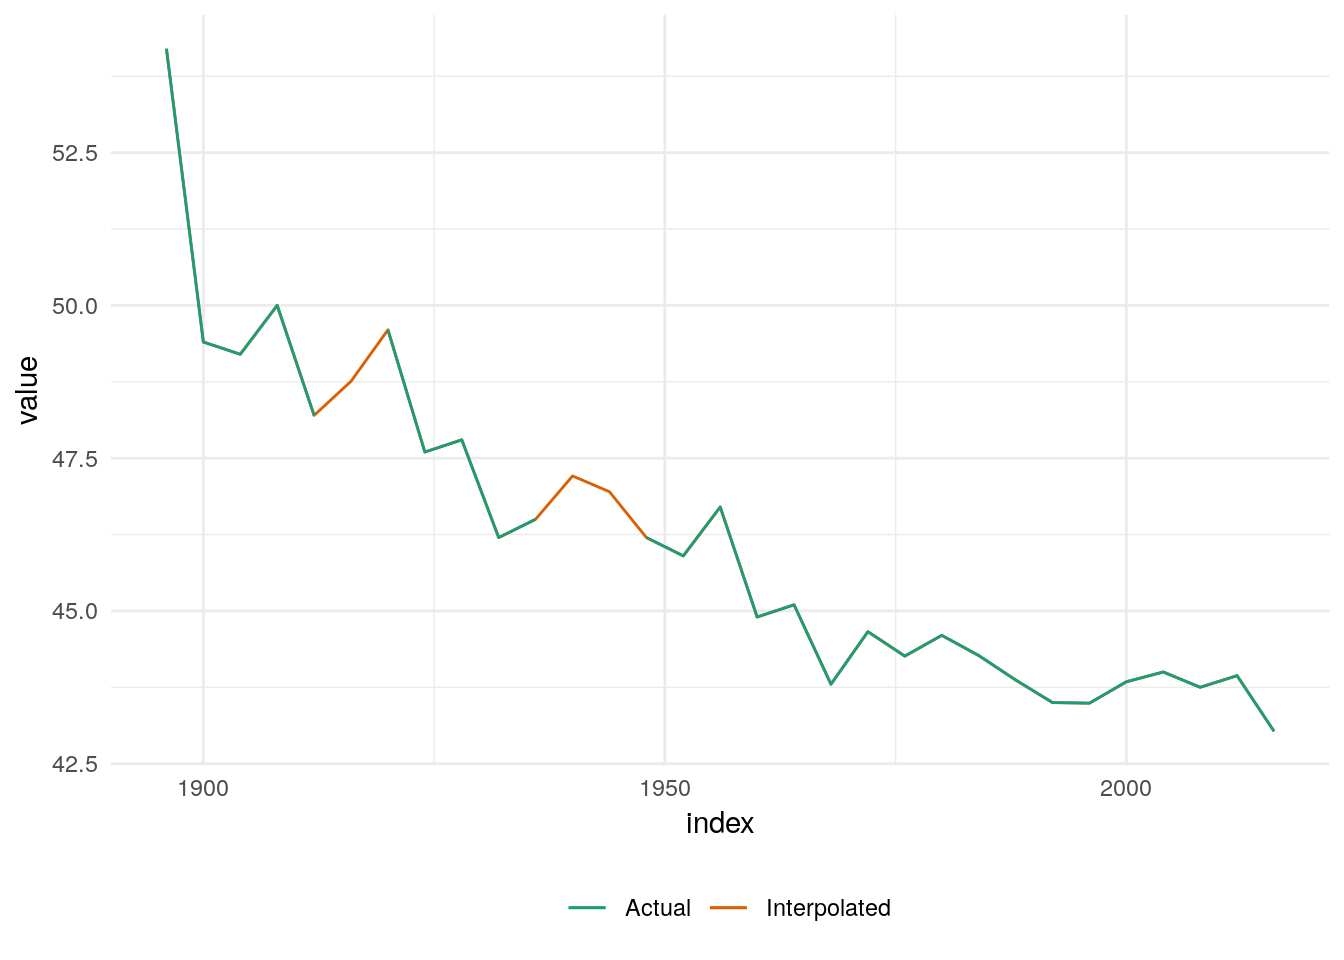
\includegraphics{tidy-forecasting_files/figure-latex/mens400-interpolated-display-1.pdf}

\hypertarget{re-estimation}{%
\section{Re-estimation}\label{re-estimation}}

\url{https://github.com/tidyverts/fable/issues/43}

\hypertarget{refit}{%
\subsection{refit()}\label{refit}}

The refitting a model allows the same model to be applied to a new dataset. This is similar to the \texttt{model} argument available in most modelling functions from the \href{https://github.com/robjhyndman/forecast/}{forecast package}.

The refitted model should maintain the same structure and coefficients of the original model, with fitted information updated to reflect the model's behaviour on the new dataset. It should also be possible to allow re-estimation of parameters using the \texttt{reestimate} argument, which keeps the selected model terms but updates the model coefficients/parameters.

It is expected that a refit method uses a fitted model and replacement data to return a mable.

For the ETS model for \texttt{mdeaths} estimated above:

\begin{Shaded}
\begin{Highlighting}[]
\KeywordTok{library}\NormalTok{(fable)}
\NormalTok{ets_fit <-}\StringTok{ }\KeywordTok{as_tsibble}\NormalTok{(mdeaths) }\OperatorTok\StringTok{ }
\StringTok{  }\KeywordTok{model}\NormalTok{(}\KeywordTok{ETS}\NormalTok{(value))}
\end{Highlighting}
\end{Shaded}

We may be interested in using the same model with the same coefficients to estimate the \texttt{fdeaths} series:

\begin{Shaded}
\begin{Highlighting}[]
\KeywordTok{refit}\NormalTok{(ets_fit, }\KeywordTok{as_tsibble}\NormalTok{(fdeaths))}
\end{Highlighting}
\end{Shaded}

\begin{verbatim}
## # A mable: 1 x 1
##   `ETS(value)`
##   <model>     
## 1 <ETS(M,A,A)>
\end{verbatim}

\hypertarget{stream}{%
\subsection{stream()}\label{stream}}

Streaming data into a model allows a model to be extended to accomodate new, future data. Like \texttt{refit}, \texttt{stream} should allow re-estimation of the model parameters. As this can be a costly operation for some models, in most cases updating the parameters should not occur. However it is recommended that the model parameters are updated on a regular basis.

Suppose we are estimating electricity demand data (\texttt{tsibbledata::aus\_elec}), and after fitting a model to the existing data, a new set of data from the next month becomes available.

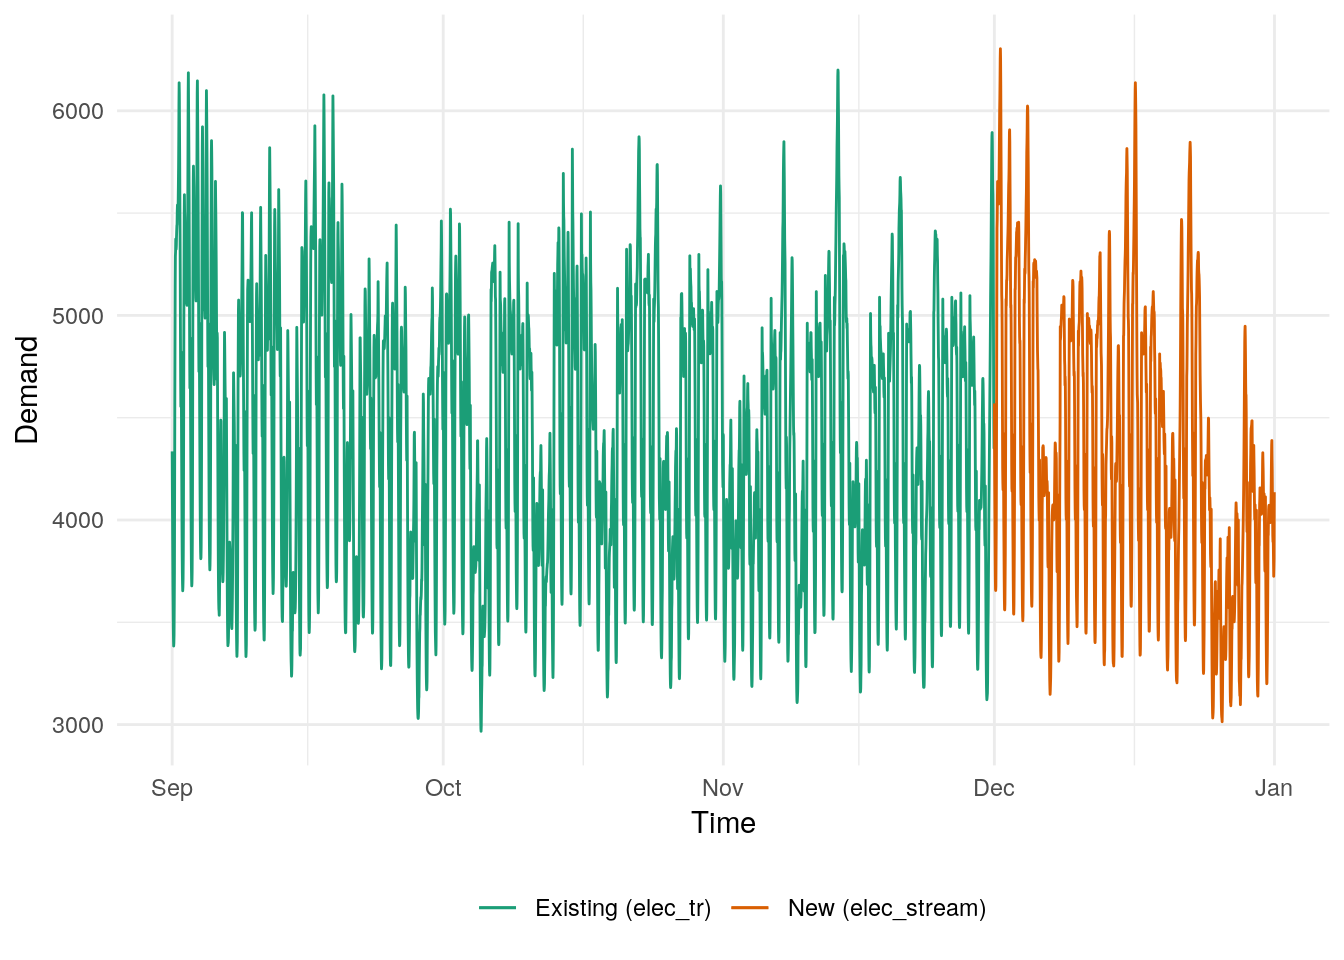
\includegraphics{tidy-forecasting_files/figure-latex/stream-tsplot-1.pdf}

A (minimal) model for the electricity demand above can be estimated using \href{https://github.com/tidyverts/fasster}{fasster}.

\begin{Shaded}
\begin{Highlighting}[]
\NormalTok{fit <-}\StringTok{ }\NormalTok{elec_tr }\OperatorTok\StringTok{ }
\StringTok{  }\KeywordTok{model}\NormalTok{(}\DataTypeTok{fasster =} \KeywordTok{fasster}\NormalTok{(Demand }\OperatorTok{~}\StringTok{ }\NormalTok{Holiday }\OperatorTok\StringTok{ }\NormalTok{(}\KeywordTok{poly}\NormalTok{(}\DecValTok{1}\NormalTok{) }\OperatorTok{+}\StringTok{ }\KeywordTok{trig}\NormalTok{(}\DecValTok{10}\NormalTok{))))}
\end{Highlighting}
\end{Shaded}

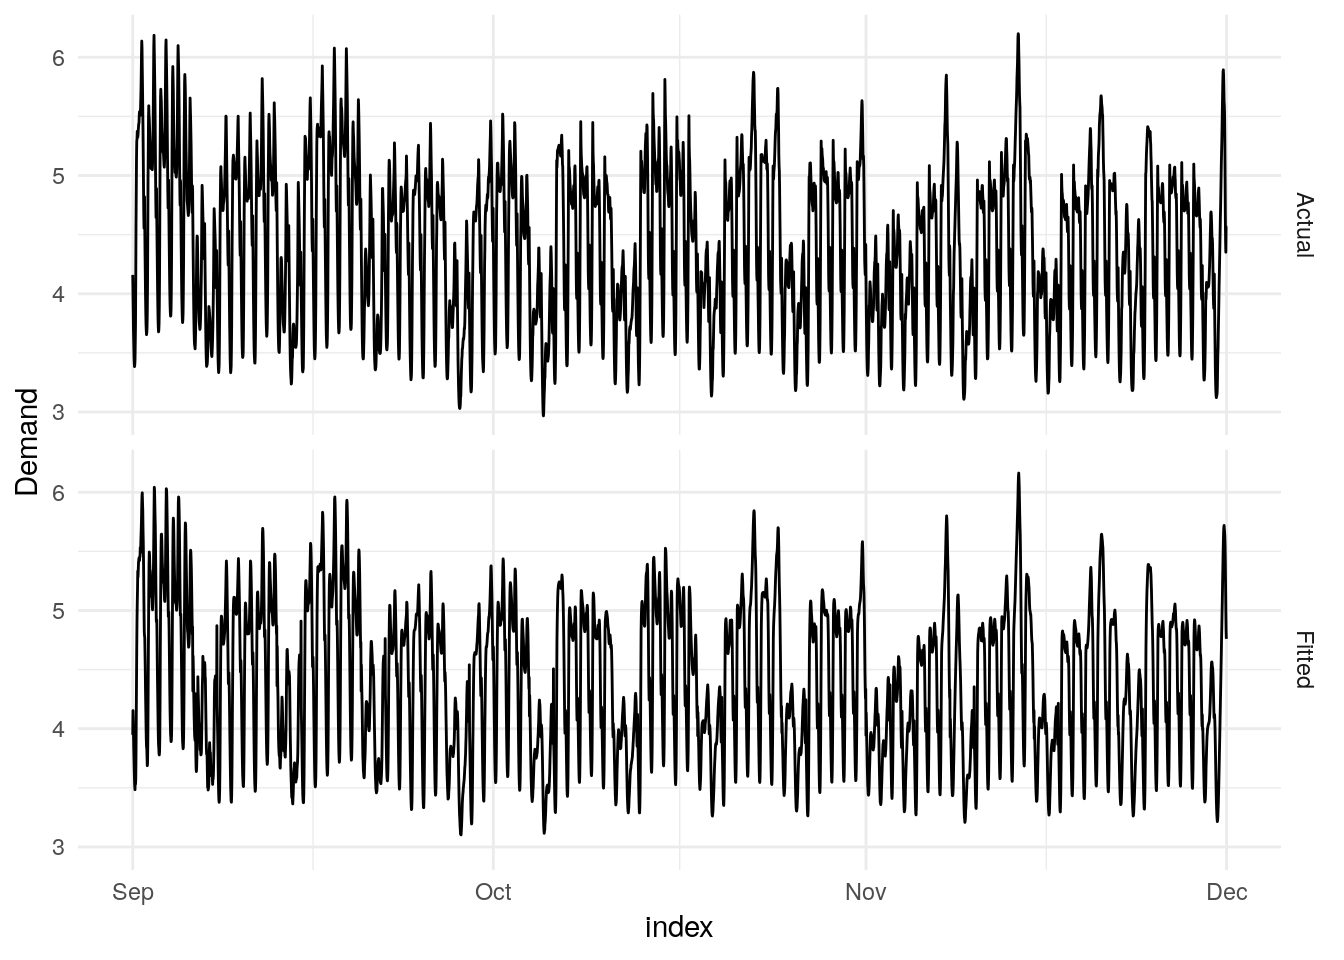
\includegraphics{tidy-forecasting_files/figure-latex/stream-fit-plot-1.pdf}

To extend these fitted values to include December's electricity data, we can use the \texttt{stream} functionality:

\begin{Shaded}
\begin{Highlighting}[]
\NormalTok{fit <-}\StringTok{ }\NormalTok{fit }\OperatorTok\StringTok{ }
\StringTok{  }\KeywordTok{stream}\NormalTok{(elec_stream)}
\end{Highlighting}
\end{Shaded}

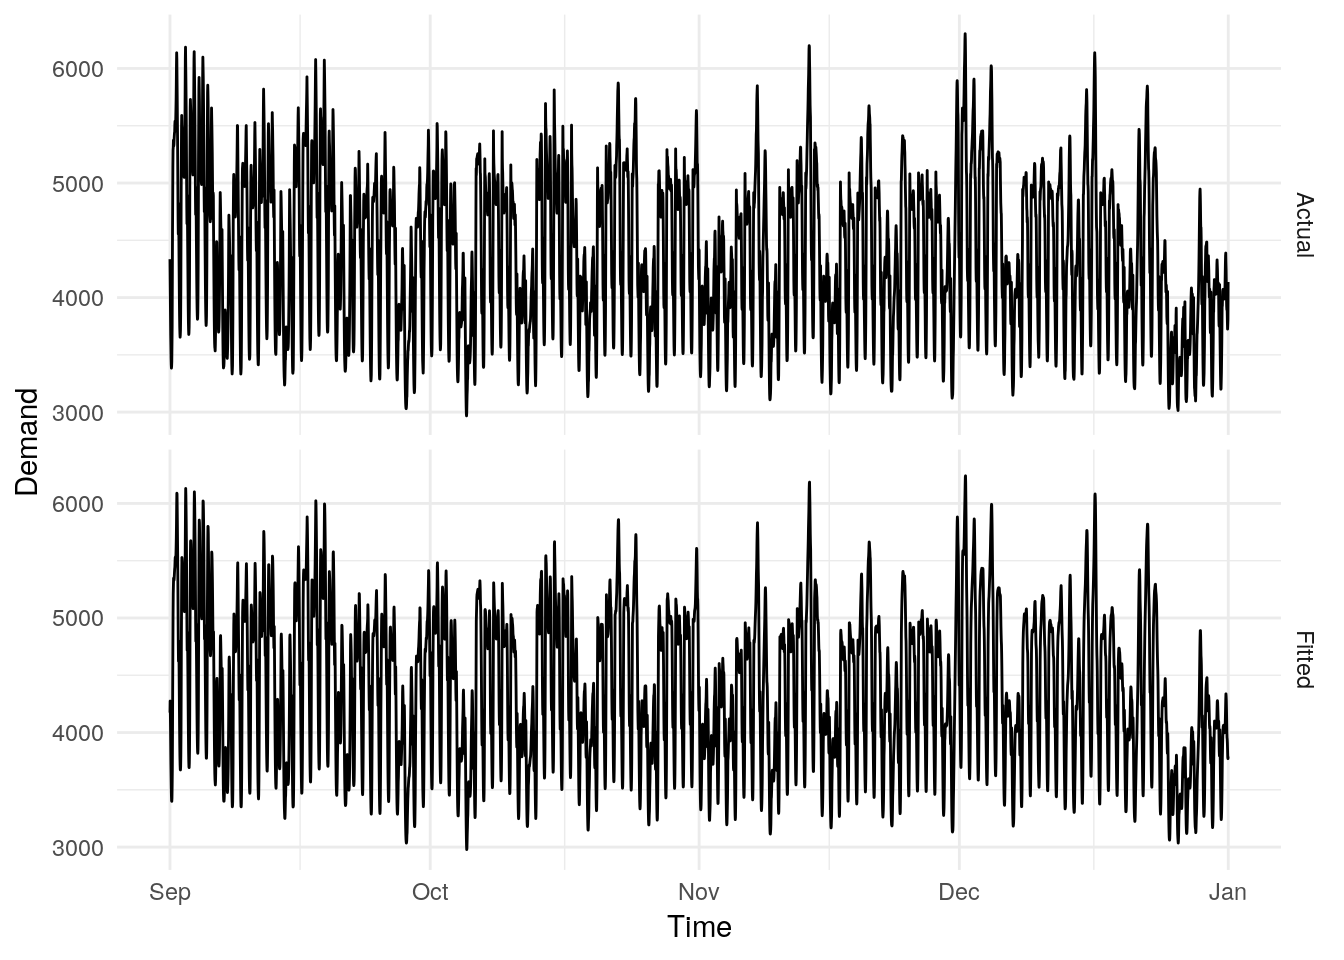
\includegraphics{tidy-forecasting_files/figure-latex/stream-plot-1.pdf}

\hypertarget{simulation}{%
\section{Simulation}\label{simulation}}

Much like the \href{https://tidymodels.github.io/model-implementation-principles/model-predictions.html\#input-data}{tidymodels opinion} toward \texttt{predict}, \texttt{generate} should not default to an archived version of the training set. This allows models to be used for simulating new data sets, which is especially relevant for time series as often future paths beyond the training set are simulated.

The generate method for a fable model should accept these arguments (names chosen for consistency with \texttt{tidymodels}):

\begin{itemize}
\tightlist
\item
  object: The model itself
\item
  new\_data: The data used for simulation
\item
  \sout{times}: The number of simulated series (handled by fablelite)
\item
  \sout{seed}: Random generator initialisation (handled by fablelite)
\end{itemize}

The \texttt{new\_data} dataset extends existing \texttt{stats::simulate} functionality by allowing the simulation to accept a new time index for simulating beyond the sample (\texttt{.idx}), and allows the simulation to work with a new set of exogenous regressors (say \texttt{x1} and \texttt{x2}).

It is expected that the innovations (\texttt{.innov}) for the simulation are randomly generated for each repition number (\texttt{rep}), which can be achieved using the \texttt{times} argument. However, users should also be able to provide a set of pre-generated innovations (\texttt{.innov}) for each repition (\texttt{.rep}). If these columns are provided in the \texttt{new\_data}, then this data will be passed directly to the simulation method (without generating new numbers over \texttt{times} replications).

\begin{verbatim}
## Warning: `id()` is deprecated for creating key.
## Please use `key = .rep`.
\end{verbatim}

\begin{verbatim}
## # A tsibble: 9 x 5 [1M]
## # Key:       .rep [3]
##    .rep     .idx .innov      x1    x2
##   <int>    <mth>  <dbl>   <dbl> <dbl>
## 1     1 2017 Jan  0.403  0.336  -1.23
## 2     1 2017 Feb  2.36   0.0252 -1.65
## 3     1 2017 Mar  0.508  4.58   -2.40
## 4     2 2017 Jan -1.52   3.28   -1.89
## 5     2 2017 Feb -0.891  0.182  -2.61
## 6     2 2017 Mar -1.47   3.73   -2.19
## 7     3 2017 Jan  1.34  -1.62   -3.02
## 8     3 2017 Feb  0.153  2.96   -1.22
## 9     3 2017 Mar -1.64   2.58   -1.66
\end{verbatim}

For the end user, creating simulations would work like this:

\begin{Shaded}
\begin{Highlighting}[]
\KeywordTok{library}\NormalTok{(fable)}
\KeywordTok{library}\NormalTok{(tsibbledata)}
\NormalTok{UKLungDeaths }\OperatorTok\StringTok{ }
\StringTok{  }\KeywordTok{model}\NormalTok{(}\DataTypeTok{lm =} \KeywordTok{TSLM}\NormalTok{(mdeaths }\OperatorTok{~}\StringTok{ }\KeywordTok{fourier}\NormalTok{(}\StringTok{"year"}\NormalTok{, }\DataTypeTok{K =} \DecValTok{4}\NormalTok{) }\OperatorTok{+}\StringTok{ }\NormalTok{fdeaths)) }\OperatorTok\StringTok{ }
\StringTok{  }\KeywordTok{generate}\NormalTok{(UKLungDeaths, }\DataTypeTok{times =} \DecValTok{5}\NormalTok{)}
\end{Highlighting}
\end{Shaded}

\begin{verbatim}
## # A tsibble: 360 x 4 [1M]
## # Key:       .rep, .model [5]
##    .model  .rep    index  .sim
##    <chr>  <int>    <mth> <dbl>
##  1 lm         1 1974 Jan 2398.
##  2 lm         1 1974 Feb 1821.
##  3 lm         1 1974 Mar 1996.
##  4 lm         1 1974 Apr 1692.
##  5 lm         1 1974 May 1406.
##  6 lm         1 1974 Jun 1375.
##  7 lm         1 1974 Jul 1110.
##  8 lm         1 1974 Aug 1003.
##  9 lm         1 1974 Sep 1009.
## 10 lm         1 1974 Oct 1466.
## # ... with 350 more rows
\end{verbatim}

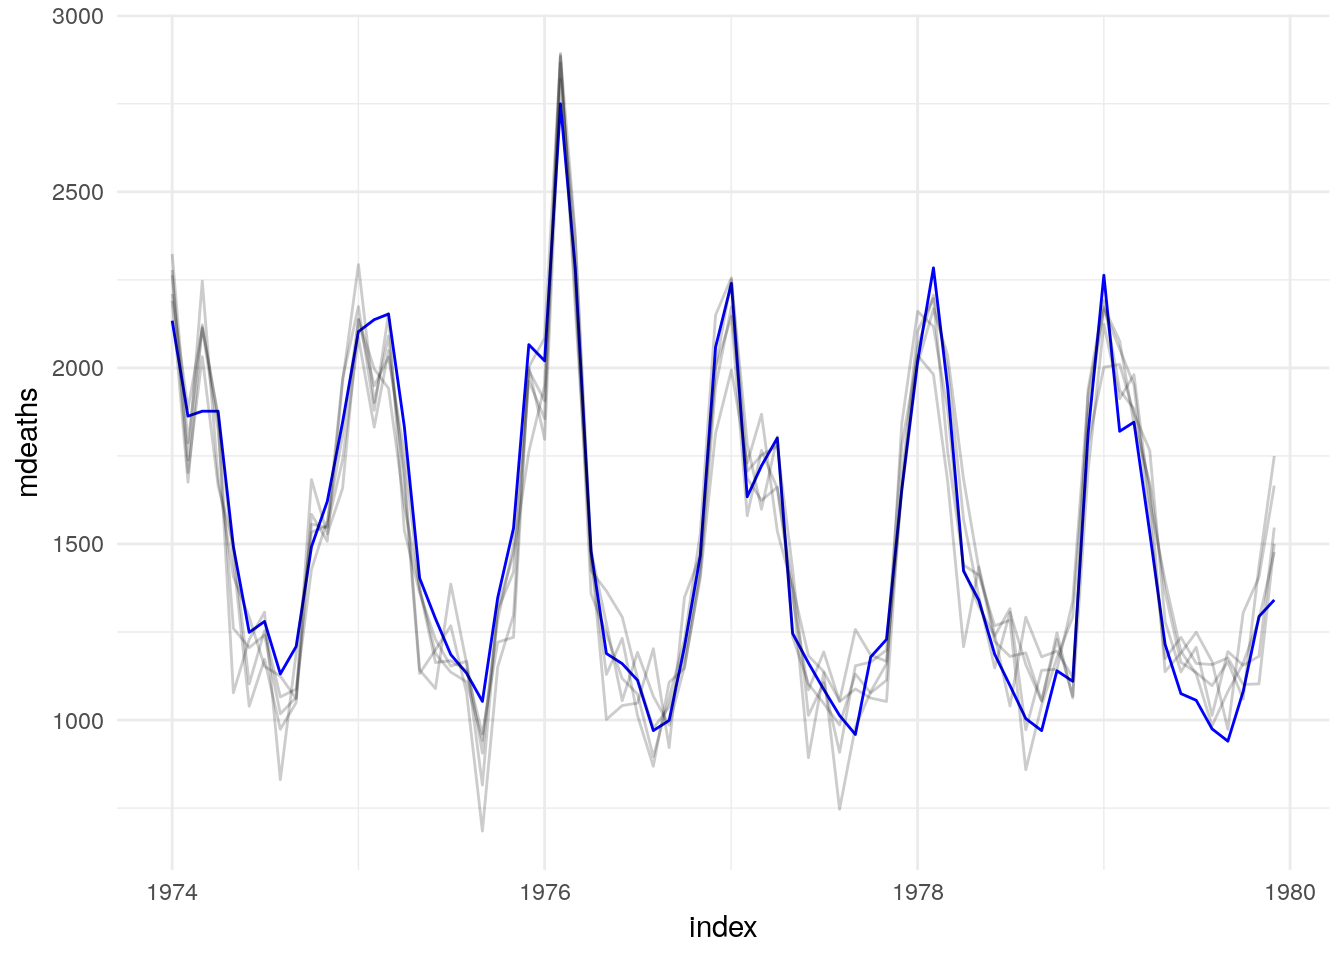
\includegraphics{tidy-forecasting_files/figure-latex/sim-example-eval-1.pdf}

Or, to generate data beyond the sample:

\begin{Shaded}
\begin{Highlighting}[]
\KeywordTok{library}\NormalTok{(lubridate)}
\NormalTok{UKLungDeaths }\OperatorTok\StringTok{ }
\StringTok{  }\KeywordTok{filter}\NormalTok{(}\KeywordTok{year}\NormalTok{(index) }\OperatorTok{<=}\StringTok{ }\DecValTok{1978}\NormalTok{) }\OperatorTok\StringTok{ }
\StringTok{  }\KeywordTok{model}\NormalTok{(}\DataTypeTok{lm =} \KeywordTok{TSLM}\NormalTok{(mdeaths }\OperatorTok{~}\StringTok{ }\KeywordTok{fourier}\NormalTok{(}\StringTok{"year"}\NormalTok{, }\DataTypeTok{K =} \DecValTok{4}\NormalTok{) }\OperatorTok{+}\StringTok{ }\NormalTok{fdeaths)) }\OperatorTok\StringTok{ }
\StringTok{  }\KeywordTok{generate}\NormalTok{(}
\NormalTok{    UKLungDeaths }\OperatorTok\StringTok{ }\KeywordTok{filter}\NormalTok{(}\KeywordTok{year}\NormalTok{(index) }\OperatorTok{>}\StringTok{ }\DecValTok{1978}\NormalTok{),}
    \DataTypeTok{times =} \DecValTok{5}
\NormalTok{  )}
\end{Highlighting}
\end{Shaded}

\begin{verbatim}
## # A tsibble: 60 x 4 [1M]
## # Key:       .rep, .model [5]
##    .model  .rep    index  .sim
##    <chr>  <int>    <mth> <dbl>
##  1 lm         1 1979 Jan 2036.
##  2 lm         1 1979 Feb 1851.
##  3 lm         1 1979 Mar 2008.
##  4 lm         1 1979 Apr 1779.
##  5 lm         1 1979 May 1343.
##  6 lm         1 1979 Jun 1207.
##  7 lm         1 1979 Jul  976.
##  8 lm         1 1979 Aug  974.
##  9 lm         1 1979 Sep 1068.
## 10 lm         1 1979 Oct 1215.
## # ... with 50 more rows
\end{verbatim}

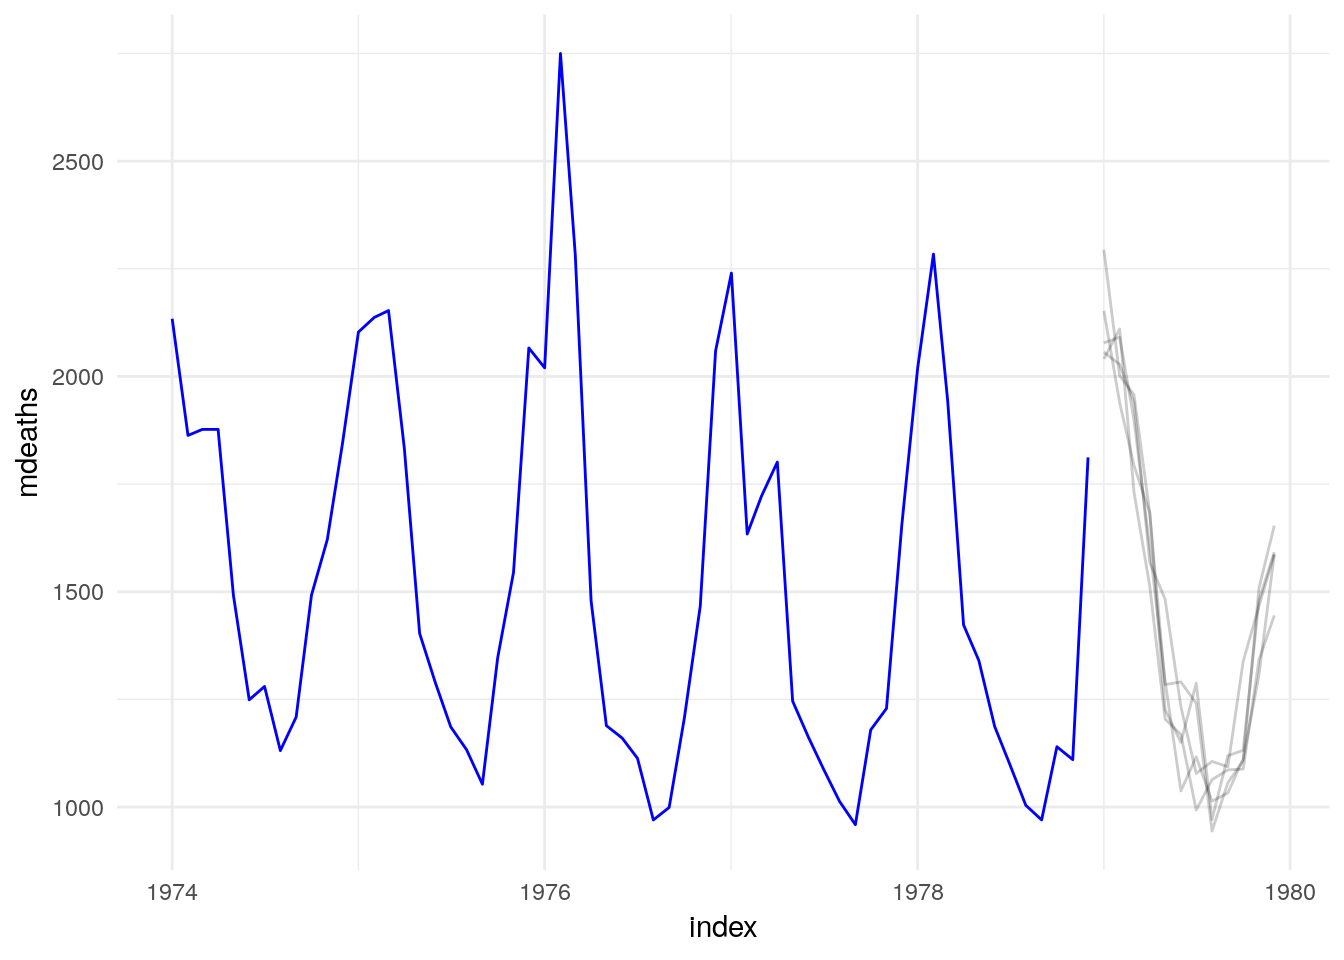
\includegraphics{tidy-forecasting_files/figure-latex/sim-future-eval-1.pdf}

\hypertarget{visualisation}{%
\section{Visualisation}\label{visualisation}}

Different plots are appropriate for visualising each type of model. For example, a plot of an ARIMA model may show the AR and/or MA roots from the model on a unit circle. A linear model has several common plots, including plots showing ``Residuals vs Fitted'' values, normality via a Q-Q plot, and measures of leverage. These model plots are further extended by the \href{http://pbreheny.github.io/visreg/}{visreg package} to show the affects of terms on the model's response. Some models currently have no model-specific plots, such as ETS, which defaults to showing a components plot using the estimated states.

Visualising these models poses a substantial challenge for consistency across models, and is made more difficult as batch modelling becomes commonplace.

\hypertarget{advanced}{%
\chapter{Advanced modelling}\label{advanced}}

\hypertarget{batch}{%
\section{Batch}\label{batch}}

\url{https://github.com/tidyverts/fable/wiki/Tidy-forecasting-with-the-fable-package}

Estimating multiple models is a \textbf{key} feature of fable. Most time series can be naturally disaggregated using a series of factors known as keys. These keys are used to uniquely identify separate time series, each of which can be modelled separately.

\begin{Shaded}
\begin{Highlighting}[]
\NormalTok{UKLungDeaths }\OperatorTok\StringTok{ }
\StringTok{  }\KeywordTok{gather}\NormalTok{(}\StringTok{"sex"}\NormalTok{, }\StringTok{"deaths"}\NormalTok{) }\OperatorTok\StringTok{ }
\StringTok{  }\KeywordTok{model}\NormalTok{(}\KeywordTok{ETS}\NormalTok{(deaths))}
\end{Highlighting}
\end{Shaded}

\begin{verbatim}
## # A mable: 2 x 2
## # Key:     sex [2]
##   sex     `ETS(deaths)`
##   <chr>   <model>      
## 1 mdeaths <ETS(M,A,A)> 
## 2 fdeaths <ETS(M,N,M)>
\end{verbatim}

\hypertarget{decomposition}{%
\section{Decomposition}\label{decomposition}}

\url{https://github.com/tidyverts/fable/wiki/Combining-models}

Objects which support a \texttt{components} method can then have their components modelled separately. The working name for this functionality is \texttt{model\_components}, however a shorter (single word) verb is preferred.

The user should be able to specify how each of the components are modelled, and the \texttt{components} method should define how each component is combined (and perhaps some default models that can be used).

\begin{Shaded}
\begin{Highlighting}[]
\KeywordTok{library}\NormalTok{(feasts)}
\NormalTok{md_decomp <-}\StringTok{ }\NormalTok{UKLungDeaths }\OperatorTok
\StringTok{  }\KeywordTok{STL}\NormalTok{(mdeaths }\OperatorTok{~}\StringTok{ }\KeywordTok{season}\NormalTok{(}\DataTypeTok{window =} \DecValTok{12}\NormalTok{))}
\NormalTok{md_decomp}
\end{Highlighting}
\end{Shaded}

\begin{verbatim}
## # A dable:           72 x 6 [1M]
## # STL Decomposition: mdeaths = trend + season_year + remainder
##       index mdeaths trend season_year remainder seas_adjust
##       <mth>   <dbl> <dbl>       <dbl>     <dbl>       <dbl>
##  1 1974 Jan    2134 1510.        594.     30.0        1540.
##  2 1974 Feb    1863 1523.        581.   -241.         1282.
##  3 1974 Mar    1877 1536.        469.   -127.         1408.
##  4 1974 Apr    1877 1549.        163.    165.         1714.
##  5 1974 May    1492 1560.       -193.    124.         1685.
##  6 1974 Jun    1249 1571.       -317.     -5.09       1566.
##  7 1974 Jul    1280 1583.       -366.     63.4        1646.
##  8 1974 Aug    1131 1593.       -466.      3.69       1597.
##  9 1974 Sep    1209 1604.       -476.     81.0        1685.
## 10 1974 Oct    1492 1615.       -243.    120.         1735.
## # ... with 62 more rows
\end{verbatim}

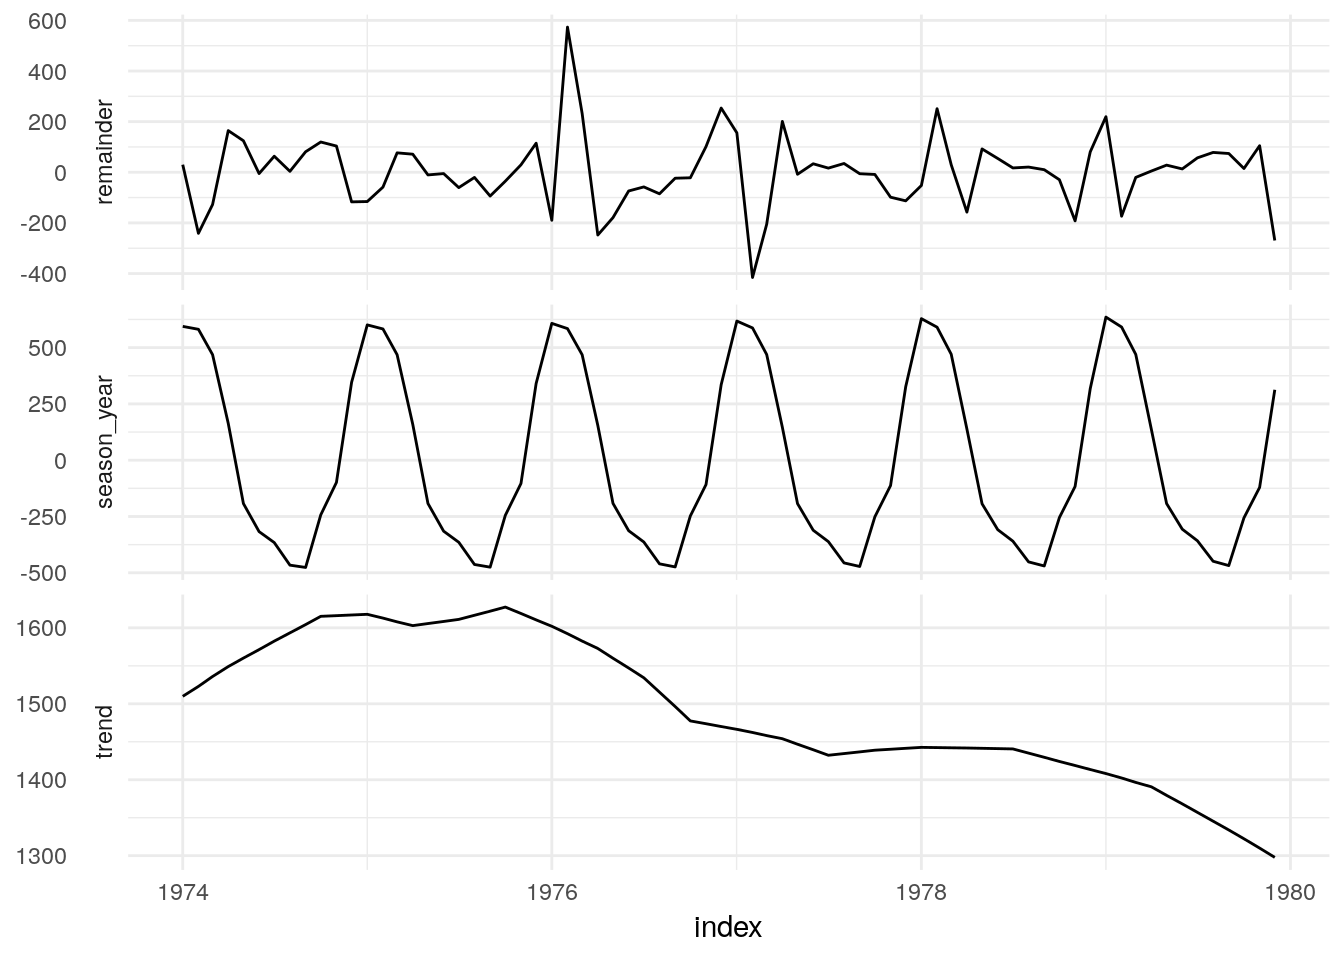
\includegraphics{tidy-forecasting_files/figure-latex/decomp-plot-1.pdf}

\begin{Shaded}
\begin{Highlighting}[]
\NormalTok{md_decomp }\OperatorTok\StringTok{ }
\StringTok{  }\KeywordTok{model_components}\NormalTok{(???)}
\end{Highlighting}
\end{Shaded}

\hypertarget{ensemble}{%
\section{Ensemble}\label{ensemble}}

\url{https://github.com/tidyverts/fable/issues/34}

\hypertarget{boosting}{%
\section{Boosting}\label{boosting}}

\hypertarget{reconciliation}{%
\section{Reconciliation}\label{reconciliation}}

\url{https://github.com/tidyverts/fable/issues/36}

\hypertarget{forecast}{%
\chapter{Forecasting}\label{forecast}}

\hypertarget{the-fable-object}{%
\section{The fable object}\label{the-fable-object}}

\begin{Shaded}
\begin{Highlighting}[]
\NormalTok{UKLungDeaths }\OperatorTok\StringTok{ }
\StringTok{  }\KeywordTok{model}\NormalTok{(}\KeywordTok{ETS}\NormalTok{(mdeaths)) }\OperatorTok\StringTok{ }
\StringTok{  }\KeywordTok{forecast}\NormalTok{()}
\end{Highlighting}
\end{Shaded}

\begin{verbatim}
## # A fable: 24 x 4 [1M]
## # Key:     .model [1]
##    .model        index value .distribution 
##    <chr>         <mth> <dbl> <dist>        
##  1 ETS(value) 1980 Jan 1957. N(1957, 34666)
##  2 ETS(value) 1980 Feb 1962. N(1962, 34842)
##  3 ETS(value) 1980 Mar 1821. N(1821, 29997)
##  4 ETS(value) 1980 Apr 1455. N(1455, 19154)
##  5 ETS(value) 1980 May 1121. N(1121, 11370)
##  6 ETS(value) 1980 Jun 1020. N(1020,  9419)
##  7 ETS(value) 1980 Jul  949. N( 949,  8151)
##  8 ETS(value) 1980 Aug  839. N( 839,  6363)
##  9 ETS(value) 1980 Sep  825. N( 825,  6165)
## 10 ETS(value) 1980 Oct 1060. N(1060, 10160)
## # ... with 14 more rows
\end{verbatim}

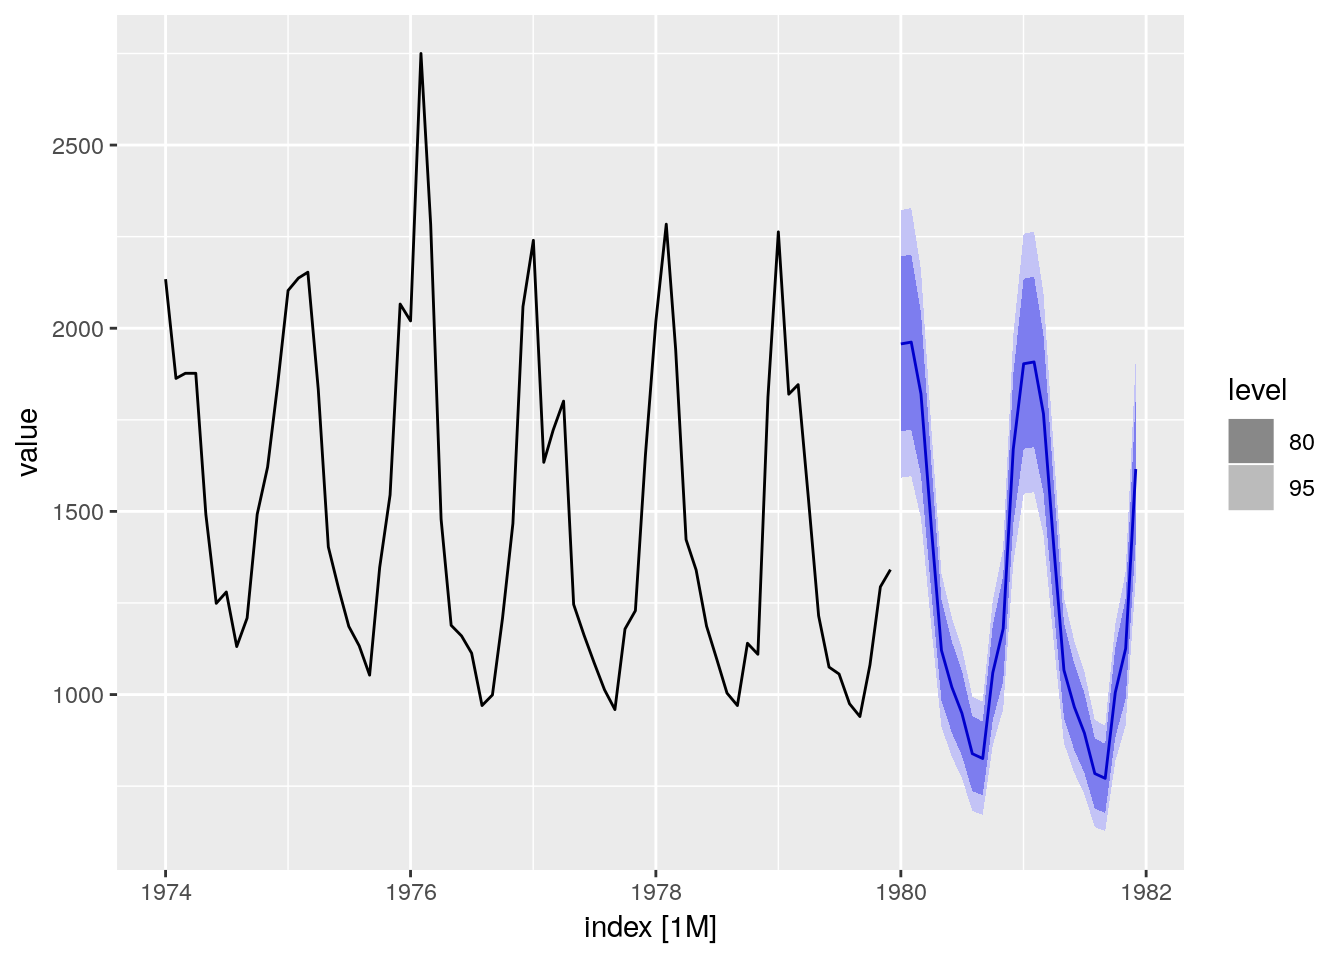
\includegraphics{tidy-forecasting_files/figure-latex/forecast-display-1.pdf}

\begin{itemize}
\tightlist
\item
  Index
\item
  Mean (backtransformed and bias adjusted)
\item
  Standard error (may not be needed)
\item
  Distribution
\end{itemize}

\hypertarget{accessing-forecasts}{%
\section{Accessing forecasts}\label{accessing-forecasts}}

\url{https://github.com/tidyverts/fasster/issues/38}

\hypertarget{bootstrapping}{%
\section{Bootstrapping}\label{bootstrapping}}

\hypertarget{visualisation-1}{%
\section{Visualisation}\label{visualisation-1}}

\begin{itemize}
\tightlist
\item
  geom\_forecast
\item
  autoplot
\item
  autolayer
\end{itemize}

\hypertarget{accuracy}{%
\chapter{Forecast evaluation}\label{accuracy}}

Where possible, the accuracy evaluation should be handled by existing tidymodels tools such as \href{https://tidymodels.github.io/yardstick/}{yardstick}. It is likely that some changes or extensions will be needed for full support of time series accuracy metrics.

\hypertarget{accuracy-1}{%
\section{Accuracy}\label{accuracy-1}}

The \href{https://github.com/robjhyndman/forecast/}{forecast package} implements accuracy as a function which is applied to a model. Out of sample accuracy can be computed by additionally providing a test set.

It is probably more transparent to compute accuracy metrics by directly providing actual response values and model predictions.

\hypertarget{model-vs-data-centric}{%
\section{Model vs data centric}\label{model-vs-data-centric}}

forecast is model centric

\begin{Shaded}
\begin{Highlighting}[]
\CommentTok{# forecast}
\KeywordTok{accuracy}\NormalTok{(}\DataTypeTok{f =}\NormalTok{ forecast, }\DataTypeTok{x =}\NormalTok{ new_ts)}
\end{Highlighting}
\end{Shaded}

yardstick is data centric
\url{https://github.com/r-lib/generics/pull/22}

\begin{Shaded}
\begin{Highlighting}[]
\CommentTok{# yardstick}
\NormalTok{fit_tbl }\OperatorTok\StringTok{ }
\StringTok{  }\KeywordTok{accuracy}\NormalTok{(col1, col2)}
\end{Highlighting}
\end{Shaded}

\hypertarget{proposed-fable-api}{%
\section{\texorpdfstring{\href{https://github.com/tidyverts/fable/issues/66}{Proposed fable API}}{Proposed fable API}}\label{proposed-fable-api}}

\hypertarget{desirable-functionality}{%
\subsection{Desirable functionality}\label{desirable-functionality}}

By default, \texttt{accuracy()} should provide a basic set of measures of fit for both models (\texttt{mdl\_df}) and forecasts (\texttt{fbl\_ts}), similarly to the \texttt{forecast} package (perhaps only MAE, RMSE/MSE, and MAPE by default).

It should be sufficiently flexible to support analysts in calculating a wide variety of accuracy measures, including:

\begin{itemize}
\tightlist
\item
  Point forecast accuracy measures
\item
  Interval accuracy measures
\item
  Distribution accuracy measures
\item
  User specified accuracy measures
\end{itemize}

The user should be able to specify which measures they wish to compute, including measures exported by \texttt{fablelite}, measures from extension packages, and user specified measures.

\hypertarget{proposed-user-interface}{%
\subsection{Proposed user interface}\label{proposed-user-interface}}

The accuracy measures to be calculated can be specified as a list of accuracy measure functions as the \texttt{measures} argument. This input will also be flattened, allowing groups of accuracy measures to be defined.

The \texttt{...} is used to provide additional arguments that will be applied to all accuracy measures (where supported).

For models (\texttt{mdl\_df}), no additional inputs are required:

\begin{Shaded}
\begin{Highlighting}[]
\NormalTok{mbl }\OperatorTok\StringTok{ }
\StringTok{  }\KeywordTok{accuracy}\NormalTok{(}
    \DataTypeTok{measures =} \KeywordTok{list}\NormalTok{(MASE, MAE, ME),}
\NormalTok{    ...}
\NormalTok{  )}
\end{Highlighting}
\end{Shaded}

For forecasts (\texttt{fbl\_ts}), the test set must be provided. Additionally, the dataset used for model training can be provided (interface still under consideration) to extend the inputs (required for MASE):

\begin{Shaded}
\begin{Highlighting}[]
\NormalTok{mbl }\OperatorTok\StringTok{ }
\StringTok{  }\KeywordTok{accuracy}\NormalTok{(}
\NormalTok{    new_data,}
    \DataTypeTok{measures =} \KeywordTok{list}\NormalTok{(MASE, MAE, ME),}
    \DataTypeTok{training_data =} \OtherTok{NULL}
\NormalTok{    ...}
\NormalTok{  )}
\end{Highlighting}
\end{Shaded}

\hypertarget{implementation-details}{%
\subsection{Implementation details}\label{implementation-details}}

To achieve this, accuracy measure functions can expect a set of basic inputs from \texttt{accuracy()}. The measures that are required for computation should be used as formals for the function. These inputs include (list is not yet comprehensive and will be added to):

\begin{itemize}
\tightlist
\item
  .resid: A vector of residuals from either the training (model accuracy) or test (forecast accuracy) data.
\item
  .resp: A vector of responses matching the residuals (for forecast accuracy, the original data must be provided).
\item
  .fitted: The fitted values from the model, or forecasted values from the forecast.
\item
  .dist: The distribution of fitted values from the model, or forecasted values from the forecast.
\item
  .period: The seasonal period of the data (defaulting to `smallest' seasonal period).
\item
  .expr\_resp: An expression for the response variable.
\end{itemize}

If a method allows more inputs than this, such as demeaning for MASE, these additional arguments are provided in the dots of the accuracy function.

\hypertarget{cross-validation}{%
\section{Cross validation}\label{cross-validation}}

\texttt{CV(tsbl,\ mdl,\ h,\ window\_type,\ ...)}

\hypertarget{visualisation-2}{%
\section{Visualisation}\label{visualisation-2}}

\hypertarget{report}{%
\chapter{Reporting}\label{report}}

\hypertarget{model-equations}{%
\section{Model equations}\label{model-equations}}

\texttt{equation()} displays a mathematical representation of the model that has been used.

\url{https://github.com/tidyverts/fable/issues/4}

\url{https://github.com/tidymodels/broom/issues/492}

(currently not implemented)

\hypertarget{object-reports}{%
\section{Object reports}\label{object-reports}}

\texttt{report()} returns a formatted summary of the object suitable for R Markdown documents and shiny applications.

(currently not implemented)


\end{document}
